%class
	\documentclass{beamer}

%template
	\usetheme{HannoverSalman}
	\setbeamertemplate{navigation symbols}{}
	%\setbeamertemplate{footline}{\centering{\insertframenumber/\insertpresentationendpage}}
	%\setbeamertemplate{footline}{\hspace*{.5cm}\scriptsize{\hfill\insertframenumber\hspace*{.5cm}}} 


%packages
	\usepackage{amsmath, amssymb, graphicx,cancel}
	\usepackage[absolute,overlay]{textpos}
	\usepackage{subfigure}
	\usepackage{caption}\captionsetup{labelformat=empty,labelsep=none}
	\usepackage{geometry}
	\geometry{verbose}
	\usepackage{color}
	\usepackage{xmpmulti}
	\usepackage[3D]{movie15}
	\usepackage{hyperref}
%	\usepackage{bookmark}
	\usepackage[open,openlevel=4,atend]{bookmark}
	%\bookmarksetup{color=blue}
	\usepackage{multirow}
	\usepackage[style=numeric,defernumbers, authoryear]{biblatex}
	%\usepackage[square,sort]{natbib}
	%\usepackage{fancyhdr}%\pagestyle{fancy} 

	
	\hypersetup{bookmarksdepth = 4}


%citations files
	\bibliography{MyCitations}

%logoCSIPCPL
    \setlength{\TPHorizModule}{1mm}
    \setlength{\TPVertModule}{1mm}
    \newcommand{\logoCSIPCPL}
    {
    	\begin{textblock}{1}(100,2) %(100,85)  for bottom
    		
\includegraphics[width=1.5cm]{figs/logo_CSIP}
    	\end{textblock}
    	
	\begin{textblock}{1}(117,1) %(117,85)  for bottom
    		
\includegraphics[width=1.0cm]{figs/logo_CPL}
    	\end{textblock} 
    }

%logo evolution
    \newcommand{\logoEvolution}
    {    	
	\begin{textblock}{1}(110,1) %(117,85)  for bottom
    		\includegraphics[width=0.65in]{figs/logo_evolution.pdf}
    	\end{textblock} 
    }

%logo Qualcomm
    \newcommand{\logoQualcomm}
    {
    	\begin{textblock}{1}(110,2) %(100,85)  for bottom
    		\includegraphics[width=1.5cm]{figs/logo_qualcomm.jpg}
    	\end{textblock}
    }
%logo Qualcomm (long)
    \newcommand{\logoQualcommllong}
    {
    	\begin{textblock}{1}(0,0) 
    		\includegraphics[width=1.25in]{figs/logo_qualcomm_long.jpg}
    	\end{textblock}
    }

%logo Tech Tower
    \newcommand{\logoTechTower}
    {
    	\begin{textblock}{1}(0,0) 
    		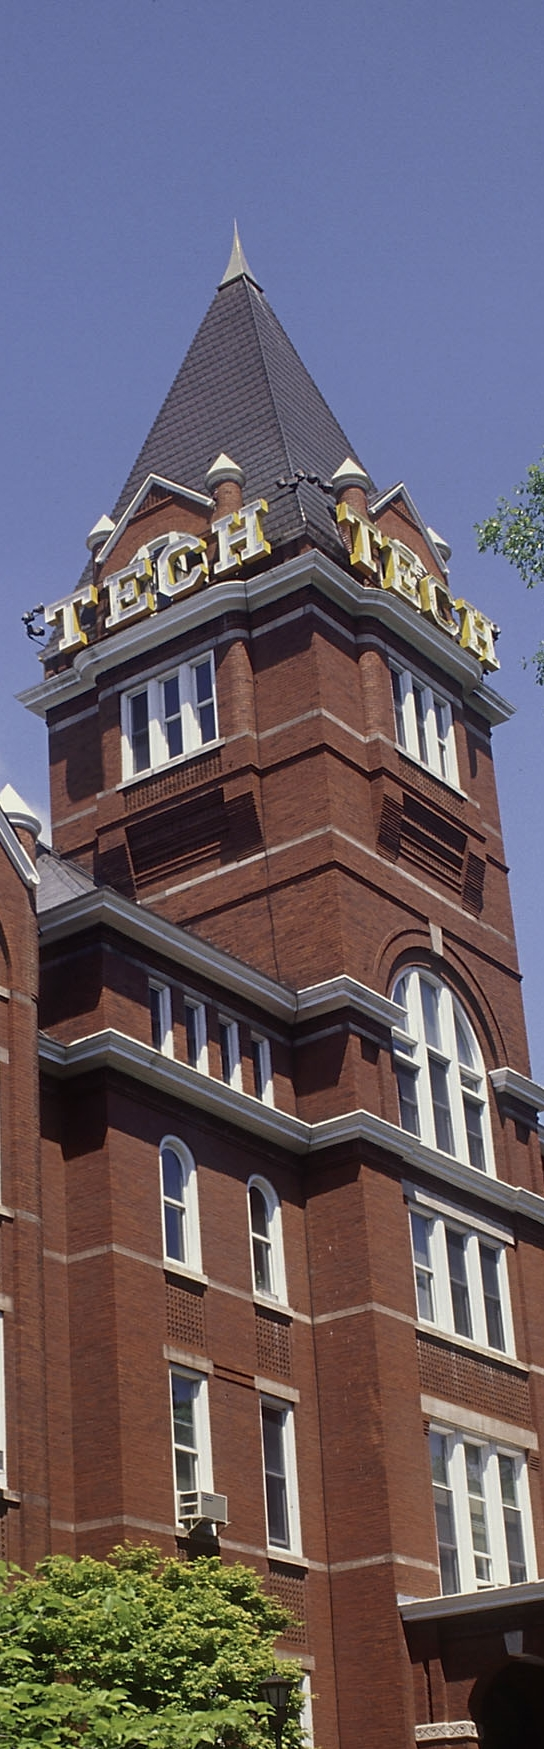
\includegraphics[width=1.25in]{figs/logo_TechTower.jpg}
    	\end{textblock}
    }

%logo tree
    \newcommand{\logoTree}
    {
    	\begin{textblock}{1}(0,0) 
    		\includegraphics[width=1.25in]{figs/logo_tree.jpg}
    	\end{textblock}
    }
%page numbers
    \newcommand{\mypagenum}
    {
    	\begin{textblock}{1}(1,94) 
		{\tiny \color[rgb]{0.2,0.2,1}\insertframenumber} %\insertframenumber,\insertpresentationendpage, \inserttotalframenumber
    	\end{textblock}
    }
%my footnote citation
	\newcommand{\myFootnoteCitation}[2]
	{
		\footnote{\tiny \citeauthor{#1}, \emph{#2}, \citeyear{#1}.}  %\citeauthor{#1}, \citetitle{#1}, #2 \citeyear{#1}.
	}
%my refer to citation
	\newcommand{\mycite}[1]
	{
		\emph{\citeauthor{#1} (\citeyear{#1})}
	}
%my footnote website citation
	\newcommand{\myFootnoteWebsiteCitation}[1]
	{
		\footnote{\tiny \citeauthor{#1}}
	}

\let\thefootnote\relax\footnotetext{Footnotetext without footnote mark}


%section underline
%\newcommand{\tmpsection}[1]{}
%\let\tmpsection=\section
%\renewcommand{\section}[1]{\tmpsection{\underline{#1}}}



%commands
	\newcommand{\likelihood}{p(Z_k| x_k) }						%likelihood
	\newcommand{\prior}{p(x_k)  } 								%prior
	\newcommand{\posterior} {p(x_k| Z_k)}						%posterior
	\newcommand{\prediction} {p(x_k| Z_{k-1})}					%prediction
	\newcommand{\update} {p(x_k|Z_k)}							%update
	\newcommand{\observations} {p(Z_k)}						%observations
	\newcommand{\prevobservations} {p(Z_{k-1})}				%previous observations
	\newcommand{\dxpk} {dx_{k-1}}							%dx_{k-1}
	\newcommand{\ChapKolm}{\int{p(x_k| x_{k-1})p(x_{k-1}|Z_{k-1})} \dxpk} %Chapman Kolmogorov

	%algorithm specific: JPDAF
	\newcommand{\likelihoodJPDAF}{p(Z_k| \chi, m, Z_{k-1}) }		%1. likelihood
	\newcommand{\priorJPDAF}{p(\chi|m, Z^{k-1}} 				%2. prior	
	\newcommand{\observationsJPDAF} {p(Z_k}					%3. observations
	\newcommand{\posteriorJPDAF} {p(\chi| Z_k)}					%4. posterior

%environments
	\newenvironment{changemargin}[2]
	{
	  	\begin{list}{}
		{
			\setlength{\topsep}{0pt}%
			\setlength{\leftmargin}{#1}%
			\setlength{\rightmargin}{#2}%
			\setlength{\listparindent}{\parindent}%
			\setlength{\itemindent}{\parindent}%
			\setlength{\parsep}{\parskip}%
		}
	  	\item[]
		}
		{\end{list}
	}
%figures

%colors
\definecolor{darkgreen}{rgb}{0,0.5,0}

%personal details
	\author{Salman Aslam}
	\institute{Advisor, Dr Christopher Barnes (ECE)\\Co-advisor, Dr Aaron Bobick (CoC)\\Georgia Institute of Technology}
	\date{}

\begin{document}



%####################################################################################################
\title{World History}
%####################################################################################################
\begin{frame}[plain]\logoTree
	\institute{}
	\titlepage
\end{frame}


\begin{frame}\frametitle{Overview}\tiny
	\tableofcontents
\end{frame}

%####################################################################################################
\section{Geologic time scale}
%####################################################################################################
\begin{frame}[plain]\mypagenum
	\begin{changemargin}{-1.3in}{0in}
		\begin{figure}
			\includegraphics[height=1.0\textheight]{figs/worldHistory_Geological_time_spiral.png}
		\end{figure}
	\end{changemargin}
\end{frame}



\begin{frame}[plain]\mypagenum
	\begin{changemargin}{-1.3in}{0in}
		\begin{figure}
			\includegraphics[height=1.0\textheight]{figs/worldHistory_Geologic_clock.jpg}
		\end{figure}
	\end{changemargin}
\end{frame}



\begin{frame}[plain]\mypagenum
	\begin{changemargin}{-1.3in}{0in}
		\begin{figure}
			\includegraphics[width=1.3\textwidth]{figs/worldHistory_Geological_Time_Scale.png}
		\end{figure}
	\end{changemargin}
\end{frame}


\begin{frame}[plain]\mypagenum
	\begin{changemargin}{-1.3in}{0in}
		\multiinclude[<+>][format=jpg, start=0, graphics={width=1.35\textwidth}]{figs/worldHistory_TectonicReconstructionGlobal}
	\end{changemargin}
\end{frame}


\begin{frame}[plain]\mypagenum
	\begin{changemargin}{-1.3in}{0in}
		\begin{figure}
			\includegraphics[width=1.3\textwidth]{figs/worldHistory_geologicTimeScale.png}
		\end{figure}
	\end{changemargin}
\end{frame}



%####################################################################################################
\section{2000-1500 BC}
%####################################################################################################
\begin{frame}[plain]\mypagenum
	\begin{changemargin}{-1.3in}{0in}
		\begin{figure}
			\includegraphics[width=1.35\textwidth]{figs/worldHistory_RandMcNallyHistomap.jpg}
		\end{figure}
	\end{changemargin}
\end{frame}

%####################################################################################################
\section{Homo Sapiens}
%####################################################################################################
\begin{frame}\frametitle{Introduction}\logoEvolution
	\begin{block}{Evolution}
		Homo erectus $\rightarrow$ archaic homo sapiens $\rightarrow$ homo sapiens\\
	\end{block}
	archaic homo sapiens: 
	\begin{itemize}
		\item 500,000  years ago
		\item Homo heidelbergensis
		\item Homo rhodesiensis
		\item Homo neanderthalensis
		\item Homo antecessor (sometimes)
		\item Survived until after 30,000 years ago, perhaps as recent as 10,000 years ago
	\end{itemize}	
	modern homo sapiens
	\begin{itemize} 
		\item 200,000 years ago
		\item 70,000 years ago, gradually marginalize "archaic" varieties
	\end{itemize}
\end{frame}



%####################################################################################################
\section{Migrations}
%####################################################################################################

\begin{frame}\frametitle{Out of Africa migration}\logoEvolution
	\begin{itemize} 
		\item starts 1,000,000 years ago\\
		Homo erectus out of Africa, across Eurasia
		\item 70,000 years ago, Homo sapiens move out of Africa 
		\item 40,000 years BCE: spread across Europe, Asia, Australia
	\end{itemize}
\end{frame}



\begin{frame}\frametitle{Out of Africa migration}\logoEvolution
	\begin{figure}
		\includegraphics[width=1.0\textwidth]{figs/worldHistory_Spreading_homo_sapiens.jpg}
	\end{figure}
\end{frame}



%topics Neolithic Revolution, Indo European expansion, Turkic expansion






%####################################################################################################
\section{DNA}
%####################################################################################################

\begin{frame}\frametitle{Mitochondrial DNA}\logoEvolution

\end{frame}


%####################################################################################################
\section{Nations}
%####################################################################################################

%========================================================
\subsection{Japan}
%========================================================
\begin{frame}\frametitle{Japan}\logoEvolution

\end{frame}

%========================================================
\subsection{Mongols}
%========================================================
\begin{frame}\frametitle{Mongols}\logoEvolution

\end{frame}

%========================================================
\subsection{China}
%========================================================
\begin{frame}\frametitle{China}\logoEvolution
	%\begin{changemargin}{-1.3in}{0in}
		\multiinclude[<+>][format=jpg, start=1, graphics={width=1.0\textwidth}]{figs/worldHistory_Territories_of_Dynasties_in_China_frame}
	%\end{changemargin}
\end{frame}

%========================================================
\subsection{Russia}
%========================================================
\begin{frame}\frametitle{Russia}\logoEvolution

\end{frame}

%========================================================
\subsection{Central Asia}
%========================================================
\begin{frame}\frametitle{Central Asia}\logoEvolution

\end{frame}

%========================================================
\subsection{Persia}
%========================================================
\begin{frame}\frametitle{Persia}\logoEvolution

\end{frame}

%========================================================
\subsection{Subcontinent}
%========================================================
\begin{frame}\frametitle{circa 300 BC}\logoEvolution
	\begin{figure}
		\includegraphics[width=1.0\textwidth]{figs/worldHistory_Chandragupta_Maurya_Empire.png}
	\end{figure}
\end{frame}

%========================================================
\subsection{Buddhism}
%========================================================
\begin{frame}\frametitle{Buddhism}\logoEvolution

\end{frame}


%========================================================
\subsection{Middle East/Biblical}
%========================================================
\begin{frame}\frametitle{Middle East/biblical}\logoEvolution

\end{frame}


%========================================================
\subsection{Islam}
%========================================================
\begin{frame}\frametitle{Islam}\logoEvolution

\end{frame}

%========================================================
\subsection{Byzantium}
%========================================================
\begin{frame}\frametitle{Islam}\logoEvolution

\end{frame}


%========================================================
\subsection{Turks}
%========================================================
\begin{frame}\frametitle{Turks}\logoEvolution

\end{frame}

%========================================================
\subsection{Greece}
%========================================================
\begin{frame}\frametitle{Greece}\logoEvolution

\end{frame}


%========================================================
\subsection{Rome}
%========================================================
\begin{frame}\frametitle{Rome}\logoEvolution

\end{frame}


%========================================================
\subsection{Spain}
%========================================================
\begin{frame}\frametitle{Spain}\logoEvolution

\end{frame}

%========================================================
\subsection{Europe}
%========================================================
\begin{frame}\frametitle{Europe}\logoEvolution

\end{frame}

%========================================================
\subsection{N. Africa}
%========================================================
\begin{frame}\frametitle{N. Africa}\logoEvolution

\end{frame}


%========================================================
\subsection{South America}
%========================================================
\begin{frame}\frametitle{South America}\logoEvolution

\end{frame}



%####################################################################################################
\section{Famous personalities}
%####################################################################################################
\begin{frame}\frametitle{Qin Shi Huang (China)}\logoEvolution
	first emperor of China
\end{frame}


\begin{frame}\frametitle{Cengiz Khan (Mongols)}\logoEvolution
\end{frame}

\begin{frame}\frametitle{Halagu Khan (Mongols)}\logoEvolution
\end{frame}

\begin{frame}\frametitle{Peter the Great (Russia)}\logoEvolution
\end{frame}


\begin{frame}\frametitle{Catherine the Great (Russia)}\logoEvolution
\end{frame}

\begin{frame}\frametitle{Stalin (Russia)}\logoEvolution
\end{frame}


\begin{frame}\frametitle{Muhammad (Middle East)}\logoEvolution
\end{frame}


\begin{frame}\frametitle{Jesus}\logoEvolution
\end{frame}




\begin{frame}\frametitle{Cyrus the Great}\logoEvolution
	\begin{figure}
		\includegraphics[width=1.0\textwidth]{figs/worldHistory_AchaemenidEmpire_Cyrus.png}
	\end{figure}
\end{frame}


\begin{frame}\frametitle{Elizabeth}\logoEvolution
\end{frame}


\begin{frame}\frametitle{Tabari}\logoEvolution
	\begin{itemize}\tiny
		\item 838-923, Iran, 20 km south of the Caspian Sea, most time in Baghdad
		\item West
			\begin{itemize}\tiny
				\item Charlemagne, emperor 800 - 814
			\end{itemize}
		\item Sunni
			\begin{itemize}\tiny
				\item Abbasids 750-1258
				\item Abd ar-Rahman II, 850
			\end{itemize}
		\item Shia
			\begin{itemize}\tiny
				\item Jafar al-Sadiq dies around 750
				\item 10th imam, Ali al-Hadi, 850
			\end{itemize}
		\item Persia
			\begin{itemize}\tiny
				\item Tahirids 821-873
				\item Alavids 864-928
			\end{itemize}
		\item China
			\begin{itemize}\tiny
				\item Tang dynasty (618-904)
				\item Tang started around Muhammad and went to Tabari
			\end{itemize}
		\item Byzantine
			\begin{itemize}\tiny
				\item Empress, Saint Theodora the Armenian, 850 
				\item Basil I, the Macedonian
				\item Leo VI, the Wise
			\end{itemize}
	\end{itemize}
\end{frame}



\begin{frame}\frametitle{Joan of Arc}\logoEvolution
\end{frame}



%####################################################################################################
%####################################################################################################
%\bibliographystyle{ieee}
%\bibliography{c:/salman/work/writing/MyCitations}
\end{document}
%####################################################################################################

%####################################################################################################


